\chapter{Supersymmetry} \label{ch:susy}

Supersymmetry (SUSY) is an extension to the Standard Model, that introduces a new spacetime symmetry relating fermionic and bosonic fields.
It is a remarkable theory, which has the potential to resolve many of the known problems of the Standard Model in one fell swoop.

\section{Motivation for New Physics}\label{sec:susy_motivation}

As described in~\ref{sec:sm_limits}, the Standard Model leaves open some very important questions.
These mysteries all point towards a more fundamental theory, one which is applicable at short distances scales,
or equivalently, higher energies.
The most important task of this new theory is to explain why the Higgs mass is so small,
in a way that avoids the extreme fine-tuning required by the Standard Model.
But a more fundamental theory of particle physics could potentially simplify the symmetry structure of the model,
and provide an explanation for the seemingly arbitrary quantum numbers of the Standard Model particles.
This new theory should not be seen as a replacement for the Standard Model, but rather an extension of it.
Whatever the new theory is, it should be applicable at very short distance scales.
And at low energies, it must reduce to the Standard Model.
We know this because all experimental evidence gathered so far indicates the Standard Model is a correct theory
up to the energy scales at which it has been probed.
In this view, the Standard Model is considered an effective field theory (EFT),
valid below the scale of new physics, $\Lambda_{NP}$.

\subsection{Naturalness}\label{subsec:susy_naturalness}

As explained in~\ref{subsec:sm_hierarchy}, the Standard Model suffers from a problem of extreme fine tuning.
Quadratic diverges in the quantum corrections to the Higgs mass-squared require the bare mass of the Higgs to be
specified to one part in $10^{19}$, which is phenomenally unlikely to happen by chance.

The quadratic divergences occur in loop diagrams,
the largest contribution coming from the top quark loop, shown in figure~\ref{fig:susy_top_loop}

\begin{figure}[h!]
    \centering
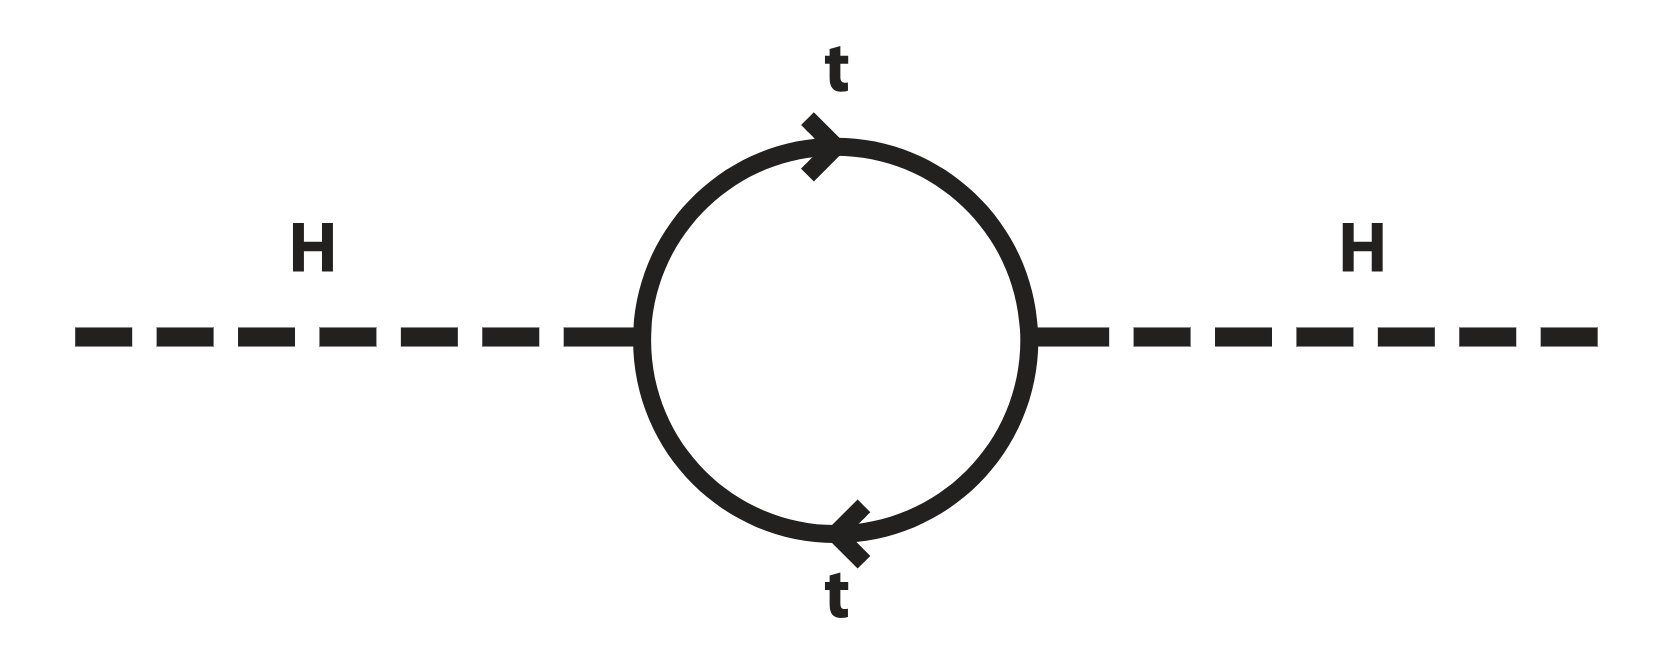
\includegraphics[width=0.6\linewidth]{susy_higgs_top_loop}
\caption{Top-quark loop diagram, the leading correction to the Higgs mass-squared. This contribution is quadratically divergent in the cutoff scale.}
\label{fig:susy_top_loop}
\end{figure}

The correction to the Higgs mass-squared coming from this diagram is:

\begin{equation}\label{eq:higgs_top_correction}
    \delta m_h^2 = \frac{3m_t^2}{2\pi^2 v^2}\Lambda_{UV}^2
\end{equation}

Where $m_t$ is the top quark mass, $v$ is the Higgs vacuum expectation value, and $\Lambda_{UV}$ is the ultraviolet cutoff.
Supersymmetry introduces a so-called superpartner for each Standard Model particle.
Standard Model fermions have bosonic superpartners, and Standard Model bosons have fermionic superpartners.
Superpartners always have the same quantum numbers as their Standard Model partners, except for spin.
The details of how this comes about will be discussed in~\ref{sec:susy_theory}.
The superpartner of the top is called the stop.
It's a scalar particle with all the same quantum numbers as the top quark, except for spin.

The introduction of superpartners leads to new quantum corrections to the Higgs mass-squared.
One of those corrections can be seen in~\ref{fig:susy_stop_loop}.

\begin{figure}[h!]
    \centering
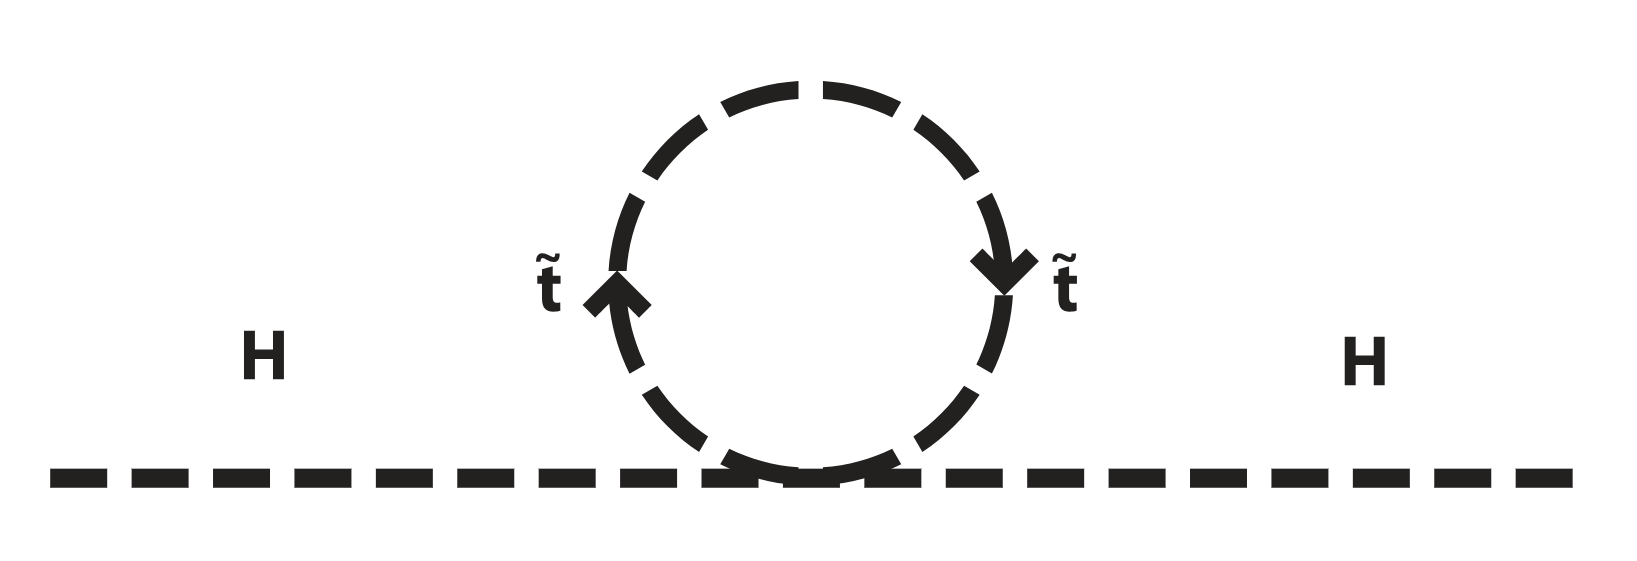
\includegraphics[width=0.6\linewidth]{susy_higgs_stop_loop}
\caption{Stop loop diagram, the leading SUSY correction to the Higgs mass-squared. This contribution is quadratically divergent in the cutoff scale.}
\label{fig:susy_stop_loop}
\end{figure}

The correction to the Higgs mass-squared coming from this diagram is:

\begin{equation}\label{eq:higgs_stop_correction}
    \delta m_h^2 = -\frac{3m_t^2}{2\pi^2 v^2}\Lambda_{UV}^2
\end{equation}

Thus, the quadratically-divergent top-loop correction is cancelled exactly.
A similar cancellation occurs for all other quadratic divergences in the calculation,
leaving terms that are only logarithmically divergent in the cutoff.

In SUSY, the leading correction to the Higgs mass-squared is proportional to the log of the cutoff scale,
and the squared difference between the top and stop masses:

\begin{equation}\label{eq:susy_higgs_correction}
    \delta m_h^2 \propto \left(m_{\tilde{t}}^2 - m_t^2\right)  \Lambda_{UV}
\end{equation}\cite{susy-pheno-2000}

The amount of fine-tuning required can be quantified by $m_h / \delta m_h $, so in order to preserve naturalness,
the stop mass cannot be much heavier than the top quark mass.
If we allow for fine-tuning of only 1 part in 10, then the stop mass shouldn't be higher than the $1~TeV$ scale,
which indicates that SUSY should be accessible by the LHC .

\subsection{Grand Unification}\label{subsec:susy_unification}


\subsection{Dark Matter}\label{subsec:susy_dark_matter}

\section{Theory and Phenomenology}\label{sec:susy_theory}

\section{R-Parity and R-parity Violation}\label{sec:susy_rpv}
